\documentclass[14pt,compress,usenames,dvipsnames,aspectratio=169]{beamer}
\setbeameroption{show notes on second screen=right}
\setbeamertemplate{note page}{\pagecolor{yellow!5}\insertnote}\usepackage{palatino}
\useoutertheme{shadow}
\usetheme{CambridgeUS}
\definecolor{mygreen}{RGB}{150, 255, 210}%186}
\definecolor{leftblue}{RGB}{230,255,255}
\definecolor{rightblue}{RGB}{111,195,223}
\definecolor{lefttron}{RGB}{19,44,65}
\definecolor{myblack}{RGB}{27,27,27}
\definecolor{mypurple}{RGB}{205,87,255}

\usecolortheme{owl}

% \setbeamercolor{section in head/foot}{fg = white,bg=black}
\setbeamercolor{title}{fg=green,bg=black}
\setbeamercolor{titlelike}{fg=yellow,bg=black}
\setbeamercolor{item}{fg=green}
\setbeamercolor{block title}{fg=white,bg=myblack!200}
\setbeamercolor{block body}{bg=normal text.bg!80}
\setbeamertemplate{blocks}[rounded][shadow=true]
\setbeamertemplate{headline}{}
\setbeamertemplate{footline}[frame number]
\setbeamercolor{normal text}{fg=white,bg=myblack}%!89.9}

%Gradient
\setbeamercolor{frametitle}{fg=green,bg=black}
\setbeamercolor{frametitle right}{fg=white,bg=gray}
\setbeamerfont{note page}{size=\tiny},

\usepackage[utf8]{inputenc}
\usepackage{amsmath}
\usepackage{amsfonts}
\usepackage{amssymb}
\usepackage{graphicx}
\usepackage{shadowtext}
\usepackage{multicol}
\usepackage[makeroom]{cancel}

\usepackage{natbib}
\usepackage{float}
\usepackage{subcaption}
\usepackage{xcolor}
\usepackage{natbib}
\usepackage{bibentry}
\usepackage{animate}
\usepackage{varwidth}
\usepackage{appendixnumberbeamer}
\usepackage{hyperref}

\usepackage{tikz}
\usetikzlibrary{shapes,arrows}

\title{\textbf{Unterwegs in der Welt der mobilen Betriebssysteme - Ein Reisebericht}}
\author{\textbf{$\varphi$}}
\date{}

\usefonttheme{professionalfonts}

\usepackage{mydefs}

\setbeamercovered{transparent} 
\setbeamertemplate{navigation symbols}{} 

\begin{document}

\setbeamercovered{invisible}

\begin{frame}[plain]
\titlepage
\note {
    ja hallo, keine Ahnung
}
\end{frame}

\begin{frame}{Agenda? oder Reiseplanung?}
    \begin{enumerate}
        \item Station 1: Android
        \item Reiseplanung 
        \item Hindernis 1: Hardbrick
        \item Station 2: LineageOS
        \item Hindernis 2: Google Play Dienste
        \item Station 3: LineageOS for microG
        \item Station 4: /e/ OS 
        \item Sidequest: Ubuntu touch 
        \item Station 5: CalyxOS 
        \item Hindernis 3: Online Banking
        \item "Sie haben ihr Ziel erreicht, das Ziel befindet sich auf der linken Seite"
    \end{enumerate}

    \note{
        \begin{itemize}
            \item hier muss nicht alles vorgelesen werden
            \item natürlich ist hier nichts vollständig oder so, halt nur alles was ich zufällig weiß/ mit was ich zufällig schon Erfahrungen gemacht habe
        \end{itemize}
    }

\end{frame}

\begin{frame}{Station 1: Android}
    Was ist eigentlich Android? 
    \begin{itemize}
        \item eigentlich ein Open Source Projekt
        \item ein Betriebssysteme für mobile Geräte
        \item “Google decided to give Android away for free and use it as a trojan horse for Google services.”
    \end{itemize}
    
    \note{
        \begin{itemize}
            \item könnte jetzt sagen ist ja logisch: das Betriebssysteme meines Smartphones, aber so einfach ist das nicht
            \item “Google decided to give Android away for free and use it as a trojan horse for Google services.”, leider keine Ahnung mehr wovon das Zitat geklaut ist.
            \item eben mit dem Ziel gegen ios zu "gewinnen", weil in etwa free to use
        \end{itemize}
    }
   
\end{frame}

\begin{frame}{Station 1: Android}
    \begin{center}
        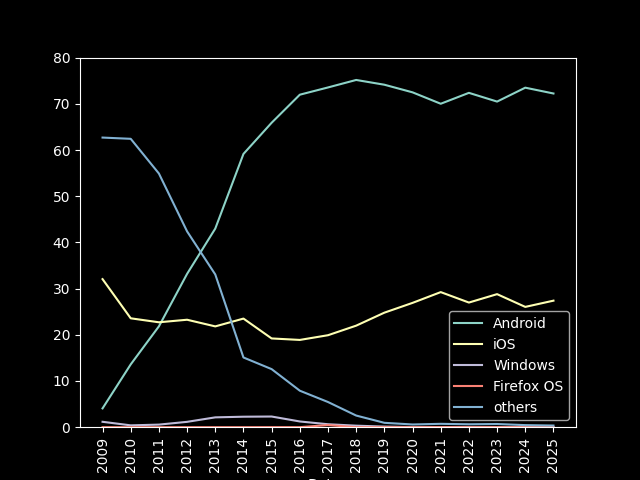
\includegraphics[width=0.66\textwidth]{Figure_1_dark.png}   
    \end{center}

    %\href{https://gs.statcounter.com/os-market-share/mobile/worldwide/#monthly-200901-202504}{quelle daten}
    
    \note{
        \begin{itemize}
            \item wird von der Open Handset Alliance entwickelt
            \item wurde von Google gegründet und wird momentan von Google geleitet
            \item Zusammenschluss von einigen (ca. 84) technologie Unternehmen
            \item alle Mitglieder sind verpflichtet default mäßig auch die GApps in “ihr Android” einzubinden
            \item Ziel: Innovation und Offenheit im mobilen Ökosystem
            \item entwickelten Android als erste offene und kostenlose Plattform für Mobilgeräte
            \item erstes Gerät mit Android war das HTC Dream, am 22.10.2008
            \item ersten “Google Geräte” war die Nexus-Produktreihe: hw von irgendwem, sw von google
            \item wurde 2016 durch Pixel ersetzt
            \item was meistens unter Android verstanden wird: der "freie Teil" inklusive dem ganzen Google Zeug oben drauf, was sich auch nicht (wirklich) Deinstallieren lässt
            \item neben dem Android für Smartphones gibt es auch (basieren alle auch auf Android):
            \item Android TV: für Fernsehgeräte (SmartTVs) optimiertes Android
            \item Wear OS:  Das Android für Smartwatches, verspricht “unkompliziertes” zusammenspielen von Uhr und Smartphone
            \item Android Auto:  Ziel: Android-Smartphone mit Infotainmentsystem des KFZs zu nutzen, Smartphone kann mittels Fahrzeuganlage bedient werden, für Navigation beispielsweise
        \end{itemize}
    }
   
\end{frame}

\begin{frame}{Station 1: Android}
    Android in etwas technischer
    \begin{columns}
        \begin{column}{0.5\textwidth}
            \begin{itemize}
                \item das was wir unter Android verstehen: AOSP mit properitären Google Anwendungen
                \item kaufe ein Gerät bekomme volle Adminrechte. Nicht so bei Android Smartphones.
                \item Quelle Bild: \href{https://source.android.com/docs/core/architecture}{AOSP}.
            \end{itemize}
        \end{column}
        \begin{column}{0.5\textwidth}  %%<--- here
            \begin{center}
                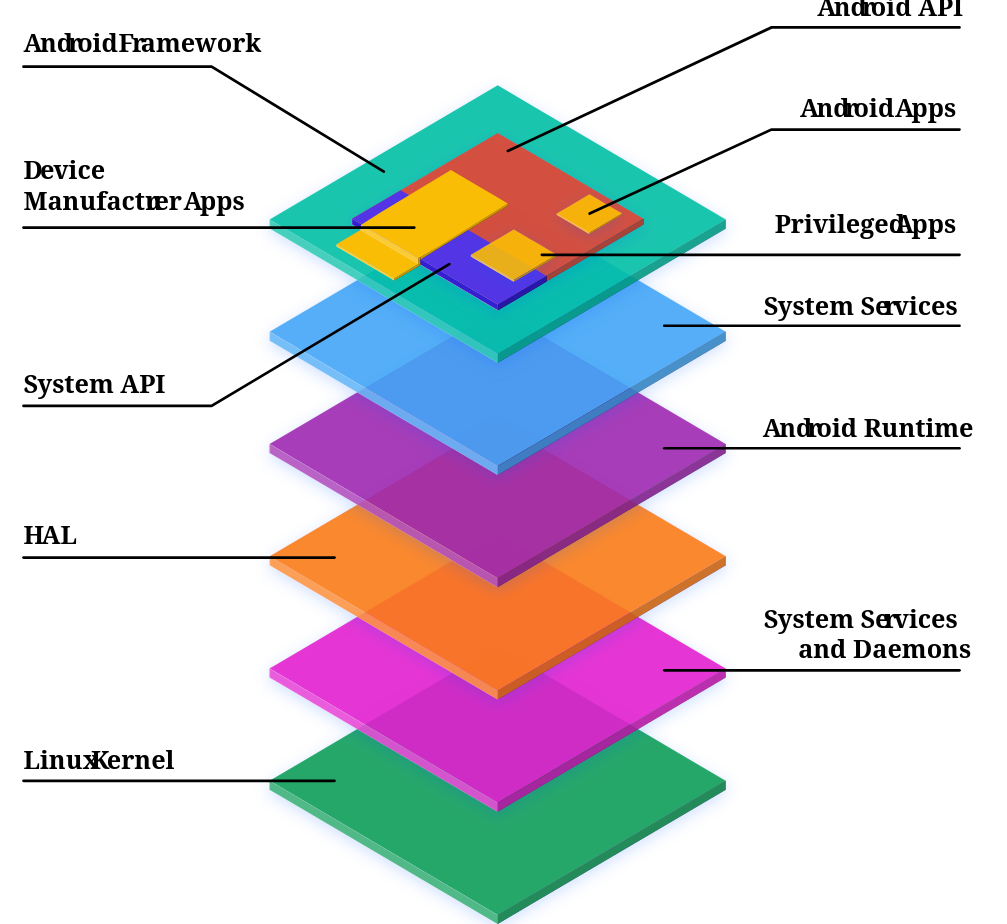
\includegraphics[width=1.0\textwidth]{Screenshot from 2025-05-09 20-58-01.png}      
            \end{center}
        \end{column}
    \end{columns}

    \note{
        \begin{itemize}
            \item auf Linux basierender Kernel (oder doch direkt Linux?)
            \item Android an sich ist freie Software (Android Open Source Project (AOSP)) unter Apache-Lizenz
            \item Google-Play-Dienste sind keine freie Software und die ganzen default google Anwendungen auch nicht
            \item Anwendungen (APPs) werden über diverse Paktemanager installiert (meistens Google Play Store)
            \item Sicherheit:
            \item SafetyNet-API prüft Kompatibilität und Sicherheit:
            \item Überprüft wird: Bootloader entsperrt? Gerät gerootet? Google-Dienste installiert? das führt dazu, dass viele APPs (Banking, etc.) auf gerooteten Geräten (mit custom-ROMs) nicht funktionieren.
            \item Abhilfen:
            \item Signatur Spoofing: Täuschungsmethoden zur Verschleierung der eigenen Identität
            \item Zygisk: Methode zur Integration von benutzerdefinierten Modulen und Root-Zugriff in den Zygote-Prozess (erster Prozess, der beim Starten des Betriebssystems ausgeführt wird) des Android-Betriebssystems, wurde im Rahmen von Magisk entwickelt, wird von der SafetyNet APi nicht erkannt, Anwendungen, die dies API verwenden, laufen weiterhin Problemlos
            \item Kernel Assisted SUperuser: Methode um Root-Rechte auf Android Geräten zu erhalten, Root-Zugriff direkt im Kernel implementiert, wird von der SafetyNet APi nicht erkannt, Anwendungen, die dies API verwenden, laufen weiterhin Problemlos
            \item normalerweise bekommt man mit dem Kauf eines Geräts auch die vollen Administrationsrechte. Bei Android nicht.
            \item Folgen: manche Anwendungen können einfach nicht deinstalliert werden, Adminrechte liegen bei Google (I guess)
        \end{itemize}
    }

\end{frame}

\begin{frame}{Station 1: Android}
    Google ist böse oder: warum ich mich auf die Reise gemacht habe.
    \begin{itemize}
        \item Hardware meines Huawei Smartphones war noch super, aber seit zu langer Zeit keine Updates mehr 
        \item gegen Monopole: alle beschweren sich immer über Apple, dass die ihr eigenes Universum aufbauen, aber Google ist auch nicht besser
        \item Ich möchte die vollen Rechte auf meinem Gerät haben.
    \end{itemize}

    \note{
        \begin{itemize}
            \item Out of live
            \item sofern die Google-Apps installiert sind, hat Google die Möglichkeit einfach Software zu löschen oder zu installieren ohne den:die Nutzer:in zu fragen; bezeichnet wird das ganze als “Sicherheitsfunktion” Remote Application Removal (daten von 2010)
            \item Google hat Kontrolle über Android: Gerätehersteller sind auf die Zusammenarbeit mit Google angewiesen
            \item Übermittlung privater Daten, bin mir nicht ganz sicher wie annonym das ganze ist (aber im Zweifel für den Angeklagten oder so)
        \end{itemize}
    }

\end{frame}

\begin{frame}{Reiseplanung}
    Was es neben stock android noch gibt (oder mögliche Reiseziele)
    \begin{itemize}
        \item ios $\to$ keine Option
        \item "freie Androids"
        \item Linux?
    \end{itemize}

    \note{
        steht eigl alles schon auf der Folie, hier gibt es nicht mehr zu sagen
    }
\end{frame}

\begin{frame}{Reiseplanung}
    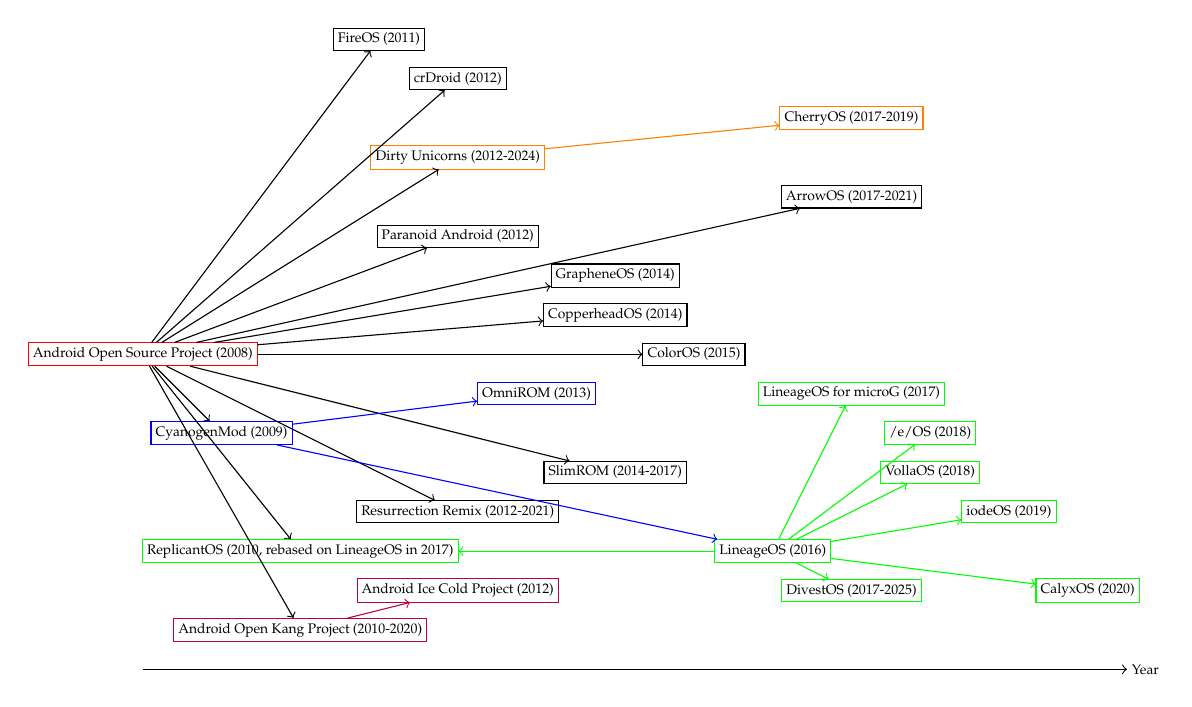
\begin{tikzpicture}[node distance=2cm, scale=0.5, transform shape]
        % Draw the year line
        \draw [->] (0,0) -- (25,0) node [right] {Year};
        
        % Draw the year labels
      %   \foreach \x in {2008, 2009, 2010, 2011, 2012, 2013, 2014, 2015, 2016, 2017, 2018, 2019, 2020, 2021, 2022, 2023, 2024, 2025}
      %   \draw (\x-2008,0) -- (\x-2008,-0.1) node [below] {\x};
        
        % Create the nodes
        \node (android) [rectangle, draw=red] at (0,8) {Android Open Source Project (2008)};
        \node (fireos) [rectangle, draw] at (6,16) {FireOS (2011)};
        \node (crdroid) [rectangle, draw] at (8,15) {crDroid (2012)};
      
        \node (dirtyunicorns) [rectangle, draw=orange] at (8,13) {Dirty Unicorns (2012-2024)};
        \node (cherryos) [rectangle, draw=orange] at (18,14) {CherryOS (2017-2019)};
      
        \node (paranoidandroid) [rectangle, draw] at (8,11) {Paranoid Android (2012)};
        \node (coloros) [rectangle, draw] at (14,8) {ColorOS (2015)};
        \node (copperheados) [rectangle, draw] at (12,9) {CopperheadOS (2014)};
        \node (arrowos) [rectangle, draw] at (18,12) {ArrowOS (2017-2021)};
      
        \node (cyanogenmod) [rectangle, draw=blue] at (2,6) {CyanogenMod (2009)};
        \node (omnirom) [rectangle, draw=blue] at (10,7) {OmniROM (2013)};
        \node (lineageos) [rectangle, draw=green] at (16,3) {LineageOS (2016)};
      
        \node (lineageos microg) [rectangle, draw=green] at (18,7) {LineageOS for microG (2017)};
        \node (eos) [rectangle, draw=green] at (20,6){/e/OS (2018)};
        \node (vollaos) [rectangle, draw=green] at (20,5) {VollaOS (2018)};
        \node (iodeos) [rectangle, draw=green] at (22,4) {iodeOS (2019)};
        \node (divestos) [rectangle, draw=green] at (18,2) {DivestOS (2017-2025)};
        \node (calyxos) [rectangle, draw=green] at (24,2) {CalyxOS (2020)};
        \node (replicantos) [rectangle, draw=green] at (4,3) {ReplicantOS (2010, rebased on LineageOS in 2017)};
      
        \node (aokp) [rectangle, draw=purple] at (4,1) {Android Open Kang Project (2010-2020)};
        \node (androidicecold) [rectangle, draw=purple] at (8,2) {Android Ice Cold Project (2012)};
      
        \node (resurrectionremix) [rectangle, draw] at (8,4) {Resurrection Remix (2012-2021)};
        \node (grapheneos) [rectangle, draw] at (12,10) {GrapheneOS (2014)};
        \node (slimrom) [rectangle, draw] at (12,5) {SlimROM (2014-2017)};
        
        \draw [->] (android) -- (replicantos);
        \draw [->] (android) -- (fireos);
        \draw [->] (android) -- (grapheneos);
        \draw [->] (android) -- (slimrom);
        \draw [->] (android) -- (resurrectionremix);
        \draw [->] (android) -- (crdroid);
        \draw [->] (android) -- (paranoidandroid);
        \draw [->] (android) -- (copperheados);
        \draw [->] (android) -- (coloros);
        \draw [->] (android) -- (arrowos);
      
        \draw [->] (android) -- (dirtyunicorns);
        \draw [->, draw=orange] (dirtyunicorns) -- (cherryos);
      
        \draw [->] (android) -- (aokp);
        \draw [->, draw=purple] (aokp) -- (androidicecold);
      
        \draw [->] (android) -- (cyanogenmod);
        \draw [->, draw=blue] (cyanogenmod) -- (omnirom);
        \draw [->, draw=blue] (cyanogenmod) -- (lineageos);
      
        \draw [->, draw=green] (lineageos) -- (divestos);
        \draw [->, draw=green] (lineageos) -- (lineageos microg);
        \draw [->, draw=green] (lineageos) -- (replicantos);
        \draw [->, draw=green] (lineageos) -- (vollaos);
        \draw [->, draw=green] (lineageos) -- (eos);
        \draw [->, draw=green] (lineageos) -- (iodeos);
        \draw [->, draw=green] (lineageos) -- (calyxos);
      \end{tikzpicture}

    \note<1>{ 
        “freie Androids”:
        \begin{itemize}
            \item dürfen alle nicht den Name Android und das Zugehörige Logo verwenden, da von Googele geschützt.
            \item China und USA kloppen sich ja gerne: kein Google auf dem Chinesischen Markt, führt du Google-Losen Androids auf Smartphones diverser Chiniesischer Hersteller (meistens nur für den Chinesischen Markt, z.B. Xiaomi mit HyperOS, Huawei mit HarmonyOS)
        \end{itemize}
        alle hier vorzulesen würde den Rahmen sprengen, paar nennenswerte spontan rauspicken\\
        aktiv:
        \begin{itemize}
            \item Volla OS: damit gibt es handys auch zu kaufen
            \item /e/OS: 2018; kommt von LineageOS; dahinter steht die gemeinnützige Stiftung “e Foundation”; es werden Smartphones mit /e/OS verkauft; standartmäßig mit microG
            \item Android Ice Cold Project: startete 2012 auf Basis von Android Open Kang Projekt (auf einem HTC Desire HD); liefert seit Android Q die Grundlage für LineageOS; Besondere FUnktionen: Erweiterbares Power-Menu, Batterieoptimierung für Google Dienste, Bootanimation ändern, SELinux Modus ändern; Nutzung von microG (Signature Spoofing wird unterstützt), …
            \item OmniROM: entsprang 2013 aus dem CyanoenMod; microG, einfache Beschränkungen der App-Berechtigungen
            \item Paranoid Andorid: 2012, eine der ältesten Custom-ROMs
            \item GraphenOS
            \item CalyxOS: 2020, von LineageOS; Datenschutz, Sicherheit, Barrierefreiheit, unkomplizierte Installation; Calyx Institute; microG ist wahlweise integriert; bootloader wird nach installation wieder gelockt; paar Datenschutzerweiterungen: Dtatusleistenindikatoren für aktive Kamerea und Mikrophon, verschlüsselte Backups, Einschränkung des Netzwerkzugriffs einzelner Apps
            \item LineageOS: 2016 fork von CyanogenMod; free from unnecessary software often pre-installed by a phone’s manufacturer or carrier that is considered to be bloatware;
            \item LineageOS forks: divestOS (ziel: mehr sicherheit und privacy, support für ältere geräte, gestorben ende 2024); /e/ (microG nativ); iodéOS (microG); LineageOS for microG; replicant (100\% frei, alle non-free Treiber weg); CalyxOS
            \item LineageOS for microG
            \item Replicant: ersetzt, vermeidet alle properitären Komponenten; hatte eine assembly auf dem 37C3
            \item crDroid
            \item iodéOS
            \item CopperheadOS: direkt von Andorid (AOSP), ca. 2015; Hersteller ist Copperhead Ltd. (ein in Toronto ansässiges Unternehmen)
        \end{itemize}
    }
    \note<2>{
        eingestellte Projekte:
        \begin{itemize}
            \item Android Open Kang Project: 2011;  wurde basierend of das Android Open Source Projekt gestartet; Der Name ist eine Kombination mit dem Wort Kang (Slang für gestohlenen Code) und AOSP (Android Open Source Project). Der Name war ursprünglich ein Witz, blieb aber bestehen
            \item Arrow OS
            \item CyanogenMod: 2009 (auf einem HTC Dream, da 2008 eine Methode gefunden wurde um Root-Zugriff auf das Linux-Subsystem zu erlangen), mittlerweile eingestellt; stammt direkt von Android ab; 2016 eingestellt, direkter Nachfolger ist LineageOS; Unterschides zu herkömmlichen Android: Privacy Guard (Beschränkung der Zugriffsrechte für einige Apps, …); Ende September 2009 schickte Googles Rechtsabteilung CyanogenMods Hauptentwickler Stefanie Kondik eine Abmahnung.; rechtlich problematisch ist die Einbindung von G-Apps in freie SW (laut Google) und die properitären Treiber
            \item Dirty Unicorns: 2012; ersten Versionen Basierten auf AOKP, dannach OmniROM; Seit Android Lollipop wurde AOSP als basis verwendet; Besonderheiten: keine Spenden, alles freiwillig
            \item DivestOS: war soft-fork von LineageOS (2014); eingestellt 2024; sind signiert, d.h. Bootloader kann auf vielen Geräten erneut gesperrt werden
            \item Resurrections Remix OS: 2012, direkt von Android (erste Version basiert auf Android 4.0)
            \item SlimRom: 2012, direkt von Android; Privacy Guard, Root-Rechte
        \end{itemize}   
        auf Android bassirende properitäre Betriebssysteme:
        \begin{itemize}
            \item Fire OS (Amazon): statt den Google diensten halt amazon äquivalente dienste
            \item Funtouch OS: 2013 von Vivo für Vvo smartphones
        \end{itemize} 
        ganz andere:
        \begin{itemize}
            \item UbuntuTouch: mobile Benuteroberfläche von Ubuntu; theoretisch in Sandbox auch Support für Android Apps; ich habe da so gar nichts zum laufen bekommen
            \item PinePhone: da läuft einfach linux drauf
            \item Linux: SailfishOS
            \item Microsoft Windows Phone oder dann Windows 10 Mobile; hat Microsoft dann eingestellt, sehr geringer Makrtanteil
            \item Firefox OS: Linux, 2012; wurde 2016 eingestellt; Ziel war quelloffene Alternative zu Android usw.
        \end{itemize}        
    }

\end{frame}

\begin{frame}{Hindernis 1: Hardbrick}
    oder mein erster Versuch ein Smartphone zu rooten
    \begin{itemize}
        \item da gibt es nicht viel zu sagen, war ungeschickt
    \end{itemize}

    \note{
        alles steht schon auf der Folie
    }
\end{frame}

\begin{frame}{Station 2: LineageOS}
    Google play Dienste, kaputtes Update und was sonst noch so los war
    \begin{itemize}
        \item wie Ubuntu, wenn man sich das erste mal mit Alternativen zu Windoof beschäftigt landet man irgendwie da, so ist das mit LineageOS auch 
        \item keine Google Play Dienste und auch kein microG
        \begin{itemize}
            \item quelloffene, via reverse engineering geschaffene Implementierung der Google Play Dienste 
            \item Framework für vollständig kompatible Android-Distributionen ohne properitäre Google-Komponenten
        \end{itemize}
        \item bisschen Kampf gehabt um alles dann zum Laufen zu bringen und genau dann kommt das erste LineageOS Update und ich hänge beim reboot in der boot loop fest
    \end{itemize}

    \note{
        eigl steht alles schon auf der Folie, abgesehen von microG
        \begin{itemize}
            \item quelloffene, via Reverse Engineering geschaffene Implementierung der Google Play Dienste
            \item “Framework um vollständig kompatible Android-Distribution ohne properitäre Google-Komponenten zu erstellen”
            \item wird von der /e/ Foundation unterstützt (seit 2020)
            \item wurde 2019 vom Prototyp Fund des Bundesministeriums für Bildung und Forschung gefördert
        \end{itemize}
    }

\end{frame}

\begin{frame}{Hindernis 2: Google Play Dienste}
    oder warum funktioniert die Hälfte nicht mehr?
    \begin{itemize}
        \item Gruppe an properitären Hintergrunddiensten und APIs, für Android Geräte (von Google entwickelt)
        \item senden permanet Daten an Google
        \item Maps und Logins 
        \item Endgegner: SaftyNet
    \end{itemize}

    \note{
        \begin{itemize}
            \item Gruppe an properitären Hintergrunddiensten und APIs, für Android Geräte (von Google entwickelt)
            \item Google Play Game: Interaktionen mit anderen Spieler:innen
            \item Saved Games: Spielstände in Google Cloud speichern
            \item Location APIs: abstrahieren verwendete Ortungstechnologien und bieten Geofencing-APIs zum Auslösen bestimmter Aktionen beim betreten/verlassen bestimmter Gebiete
            \item Fused Location Provider: Smartphone mit weniger Akkuverbrauch zu orten
            \item Aktivitätserkennung: Aktivitäten die Nutzer:in tut werden automatisch erkannt, z.B. Fahrradfahren
            \item Google Maps Android API: native Einbinden von Google Maps oder Street View in Applikationen
            \item Google Drive Android API: Zugang zu Google Drive
            \item Google Cast Android: Streaming Funktionalität
            \item Google Mobile Ads: Monetarisierung in Apps durch Googles Werbenetzwerk mit Googles Targeting-Werkzeugen
            \item Google Wallet Instant Buy: Einkaufen mit Google Wallet
            \item Autentifizierungsmethoden über das Google Konto
            \item Google Analytics: Web Analytics Dienst von Goolge; Herkunft von Besucher:innen von Websites, Verweildauer, Nutzung von Suchmaschinen, …; wird von etwa 50 bis 80\% aller Websites verwendet; “Arbeitet mit Google Ads zusammen”
            \item Google Play Protect: Sicherheitssystem
            \item SaftyNet: kann überprüfen ob Systemdateien modifiziert wurden; theoretisch dient es dazu um Manipulationen an der Firmware zu erkennen; Apps können das mithilfe von SaftyNet überprüfen lassen (um Gefahren einschätzen zu können (oder so))
            \item vielzahl von Apps funktioniert nur noch mit Google Play Diensten (also vorallem die GApps)
            \item Alle, die Google-Play-Dienste verwenden wollen (in SW oder auf Gerät) müssen Vertrag mit Google abschliesen (bindet sie dann an Google/Android)
            \item Weiterhin senden die Google-Play-Dienste permanent den Standort sowie personenbezogene Daten an Google. Es entstehen detaillierte Tagesprotokolle, die jahrelang bestehen können.
            \item Den Programm-Code dieser Bibliotheken hält Google allerdings unter Verschluss. Daher sind Apps mit solchen Bestandteilen niemals vollständig quelloffen (Open Source). Dieser Umstand wurde im Zusammenhang mit der Corona-Warn-App von Datenschützer*innen kritisiert. Die App selbst ist zwar quelloffen, allerdings ist sie auf eine Schnittstelle von Google angewiesen, für die die App Google Play-Dienste benötigt wird.
            \item Gebündelt in der App “Google Play Services”, welche defautlmäßig alle Recht hat
            \item können tatsächlich disabled werden
        \end{itemize}
    }

\end{frame}

\begin{frame}{Station 3: LineageOS for microG}
    \begin{itemize}
        \item naja also wie ich eben auch zum ersten mal zu Linux gekommen bin, wenn ein Update nicht erfolgreich ist, probiert man was neues aus
        \item kaum Unterschiede, microG ist defaultmäßig dabei
    \end{itemize}

    \note{
        steht auch schon alles auf der Folie
    }
\end{frame}

\begin{frame}{Station 4: /e/ OS}
    \begin{itemize}
        \item /e/ Universum: alles was sonst von Google kommt durch freie Alternativen ersetzt (z.B. Nextcould anstatt Google Drive)
    \end{itemize}

    \note{
        steht auch schon alles auf der Folie
    }
\end{frame}

\begin{frame}{Sidequest: Ubuntu touch}
    \begin{itemize}
        \item einfach nein
    \end{itemize}

    \note{
        UbuntuTouch: mobile Benuteroberfläche von Ubuntu; theoretisch in Sandbox auch Support für Android Apps; ich habe da so gar nichts zum laufen bekommen
    }
\end{frame}

\begin{frame}{Station 5: CalyxOS}
    \begin{itemize}
        \item Fork von LineageOS
        \item Hauptziele: Datenschutz, Sicherheit, Barrierefreiheit, unkomplizierte Installation
        \item Bootloader wird nach der Installation wieder gelockt
        \item einige Datenschutzerweiterungen: Statusleistenindikatoren für aktive Kamerea und Mikrophon, $\ldots$
    \end{itemize}

    \note{
        steht schon alles auf der Folie
    }
\end{frame}

\begin{frame}{Hindernis 3: Online Banking}
    oder wie man eine ??? Filiale lahmlegt

    \note{
        Noch nicht zu 100\% verstanden, aber: Umstellung von Tan-Generator zu App;
        die hatte erkannt, dass sie nicht aus dem Google Play Store kam;
        also App hatte nicht Funktioniert;
        lange Zeit einfach nichts passiert, Bank war auch nicht erreichbar;
        irgendwann konnte ich mich bei der App doch anmelden (App update?);
        aber zu lange gebraucht und musste einen Tan generieren um das freizuschalten und genau das konnte ich nicht;
        in der Filiale ist auch dann nichts passiert, bis die Schlange hinter mir lang genug wurde
    }
\end{frame}

\begin{frame}{"Sie haben ihr Ziel erreicht, das Ziel befindet sich auf der linken Seite"}
    Keine Ahnung wan eine Reise endet oder wann man ein Ziel erreicht hat. 
    Jedenfalls lebt es sich hier (mit CalyxOS) ganz gut.
    Bin jetzt auch am Ende.

    \note{
        steht schon alles auf der Folie
    }
\end{frame}
\end{document}